\documentclass[12pt]{article}
\usepackage{float}
\usepackage{amsmath}
\usepackage{paralist}
\usepackage{setspace}
\usepackage{listings}
\usepackage{graphicx}
\usepackage[english]{babel}
\usepackage{geometry}
\usepackage{subcaption}
\usepackage[utf8]{inputenc}
\usepackage{listings}
\usepackage{color}
\usepackage{subcaption}
\usepackage{hyperref}
\usepackage{mathtools}

\renewcommand{\figurename}{Figure}
\renewcommand{\contentsname}{Table of Contents}
\renewcommand{\refname}{Literature}


\begin{document}

\lstset
{
	language=C++,
	basicstyle=\footnotesize,
	frame=tb,
	xleftmargin=.2\textwidth,
	xrightmargin=.2\textwidth
}
\onehalfspacing
\begin{titlepage}
\begin{center}
% Oberer Teil der Titelseite:


\textsc{\LARGE University of Oldenburg}\\[1.5cm]

\textsc{\Large Fluid Dynamics II}\\[0.5cm]


% Title
\newcommand{\HRule}{\rule{\linewidth}{0.5mm}}
\HRule \\[0.4cm]
{ \huge \bfseries Turbulence Analysis}\\[0.4cm]

\HRule \\[1.5cm]

% Author and supervisor
\begin{minipage}{0.4\textwidth}
\begin{flushleft} \large
\emph{Author:}\\
Florian \textsc{B\"orgel}
Matrikelnummer: 3037497
\end{flushleft}
\end{minipage}
\hfill
\begin{minipage}{0.4\textwidth}
\begin{flushright} \large
\emph{Supervisor:} \\
Joachim \textsc{Peinke}
\end{flushright}
\end{minipage}
\\[3cm]
\vfill



% Unterer Teil der Seite
{\large \today}

\end{center}

\end{titlepage}

\tableofcontents
\newpage
\listoffigures
\listoftables

\newpage
\section{Introduction}
The aim of this exercise was to analyse different datasets for their turbulence parameters and structure. One dataset is from homogeneous isotropic turbulence and the other is measured wind data.
The provided datasets are taken from the atmosphere measured at 10 Hz and from experimental data created in a laboratory, referred to as JFM data. The JFM dataset is measured at 8000 Hz. For the JFM dataset, a hot-wire anemometer was used. It was placed at the central region of a round free air jet. \cite{markov}
This report covers the basic characteristics of the different datasets like e.g. mean value and the degree of turbulence. It also discusses the difference for alternating averaging intervals. 
The second section discusses two-point statistics. First the power-spectrum is derived and investigated. The datasets are further evaluated and compared to theoretical predictions.
Finally n-point quantities are introduced.
\section{Basis Characteristics}
The general idea to describe the motion of a fluid is to use the Navier-Stokes-Equation (NSE). However NSEs are nonlinear partial differential equations. The nonlinearity makes most problems like turbulence nearly impossible to solve analytically. Turbulence represents the time-dependent chaotic behaviour in many fluid flows. One approach to describe this turbulence is to use  statistical methods. Therefore the velocity is separated into the mean velocity and a fluctuating part. \cite{peinke}
\begin{equation}
U = u^{'} + <u>
\end{equation}
\begin{tabular}{c l}
$U$& - measured velocity\\
$u^{'}$& - fluctuating part\\
$<u>$ & - mean velocity \\
\end{tabular}\vspace{0.5cm}\\
In order to get an idea of the dataset basic one-point statistics were performed, where the mean values represents the first order moment of the dataset.
Other parameters to describe the dataset are the magnitude of fluctuation, which is the second order moment, and the degree of turbulence.
The magnitude of fluctuation is defined as:
\begin{equation}
\text{magnitude of fluctuations = } <u^{'2}>
\end{equation}
The parameter degree of turbulence gives an idea of the fluctuation in the dataset:
\begin{equation}
\text{degree of turbulence} = \frac{<u^{'2}>}{<u>^2}
\end{equation}
These operations have been performed for the given datasets are displayed in the following table:
\begin{table}[H]
\begin{tabular}{c c c c}
Datasets & mean velocity[m/s] & magnitude of fluctuation[m/s] & degree of turbulence[$\%$]\\
\hline
Atmosphere &10.45 &2.016& 0.0185 \\
JFM data & 2.25 &0.1495&0.0295\\
\end{tabular}
\caption{Basic characteristics of the given datasets}
\label{table:task_1}
\end{table}
\subsection{Probability Density Functions}
In order to visualize the wind speed distributions, a probability density function (PDF) plot was used for both datasets. PDF plots display the probability of an occurring wind speed event as the area under the curve. Therefore they can be used to check whether the first and second order moments are able to describe the one-point statistics. As discussed during the lecture only Gaussian distribution can be fully described by the first and second order moments. The outcome is shown in Figure~\ref{fig:pdf_u_both}.
\begin{figure}[H]
\begin{subfigure}{0.5\textwidth}
  \centering
  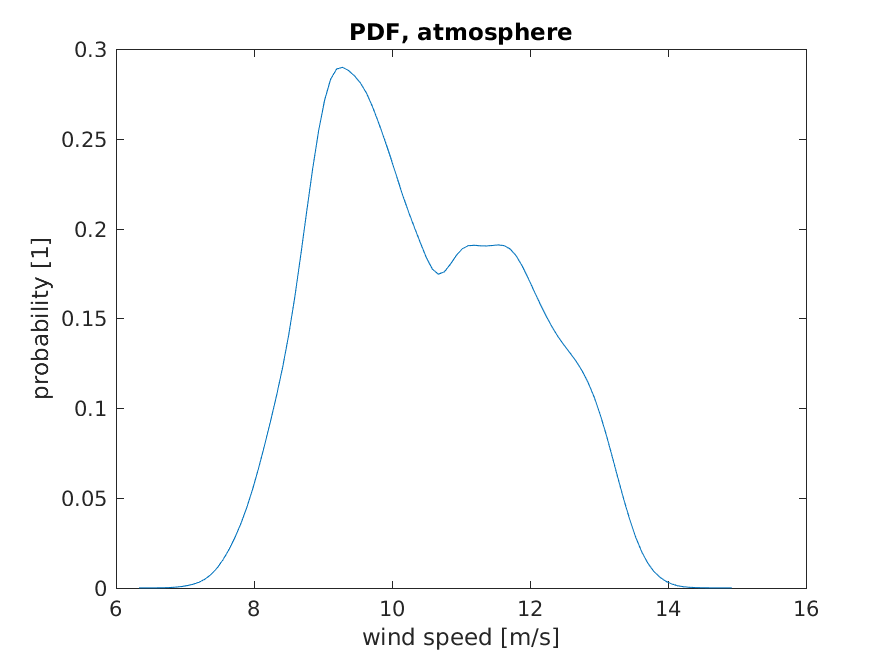
\includegraphics[width=1\linewidth]{figures/pdf_u_atmo.png}
  \caption{atmosphere}
\end{subfigure}
\begin{subfigure}{0.5\textwidth}
  \centering
  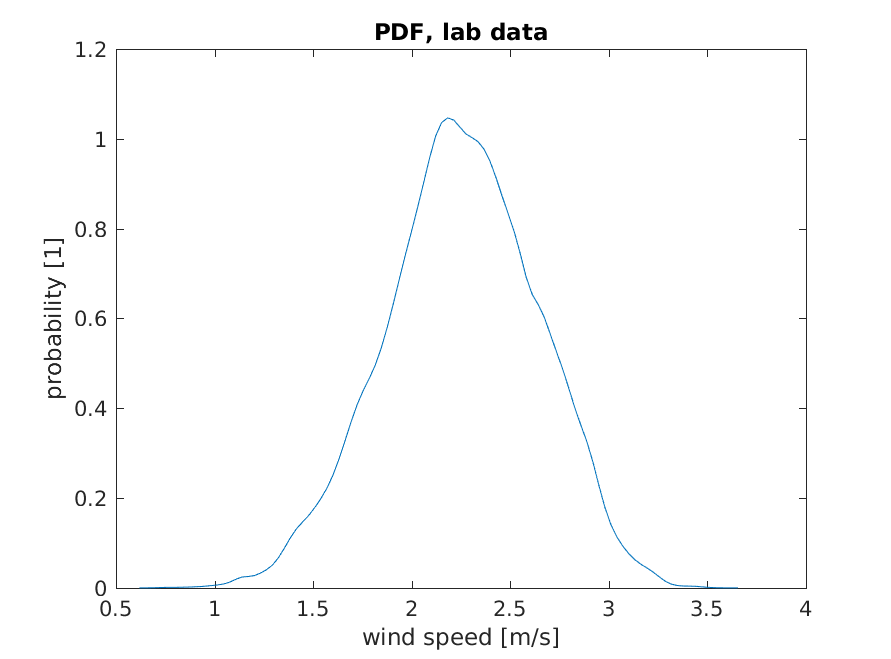
\includegraphics[width=1\linewidth]{figures/pdf_u_center.png}
  \caption{lab data}
\end{subfigure}
\caption{Velocity distribution for both datasets}
\label{fig:pdf_u_both}
\end{figure}
Figure~\ref{fig:pdf_u_both} shows that the wind distribution from the atmosphere dataset is not Gaussian distributed. In contrast the lab data shows a nearly perfect Gaussian distribution. The influence of this outcome will be further discussed in the conclusion.


It has been already mentioned that in order to describe turbulence behaviour we use statistical methods. Table~\ref{table:task_1} calculates these attributes without considering averaging intervals. It is obvious that one should consider averaging intervals because of the fluctuating behaviour of the turbulence. In the following the influence of different averaging intervals on the basis characteristics of the dataset is investigated.
Figure~\ref{fig:pdf_fluc} shows the fluctuation for different averaging intervals.

\begin{figure}[H]
\begin{subfigure}{0.5\textwidth}
  \centering
  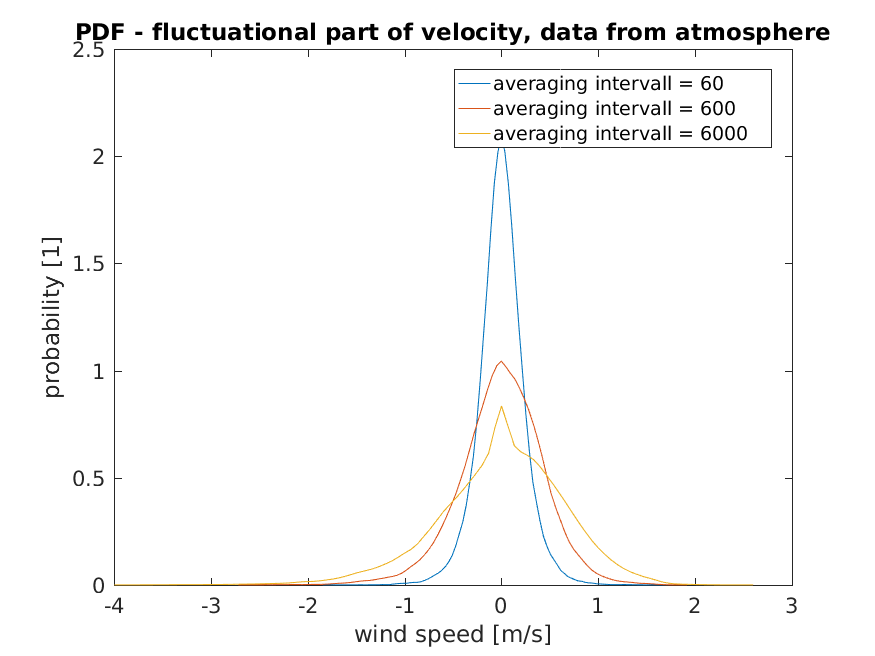
\includegraphics[width=1\linewidth]{figures/pdf_interval_comparison_atmosphere.png}
  \caption{atmosphere}
\end{subfigure}
\begin{subfigure}{0.5\textwidth}
  \centering
  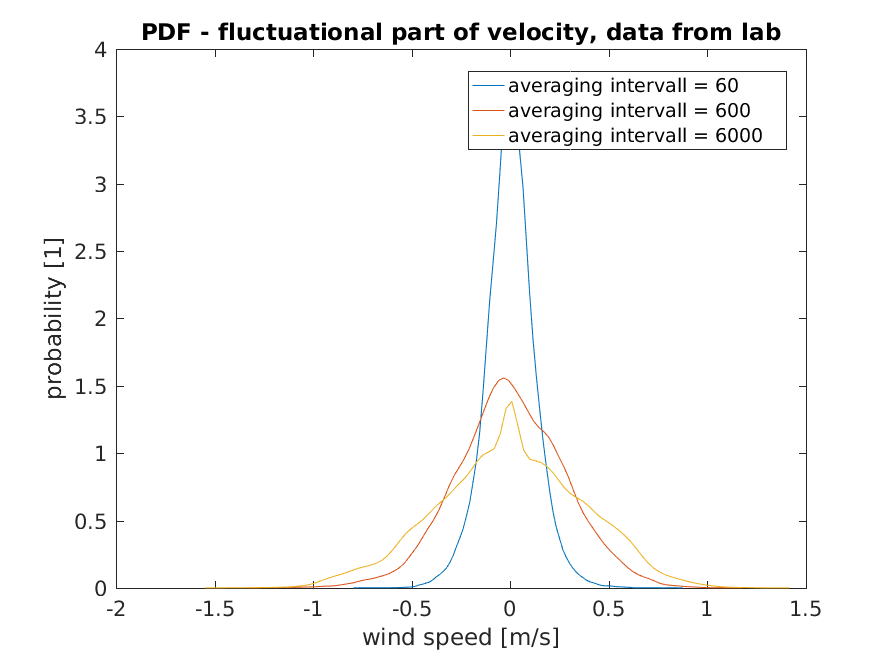
\includegraphics[width=1\linewidth]{figures/pdf_interval_comparison_labdata.png}
  \caption{lab data}
\end{subfigure}
\caption{Comparison of the fluctuation for different averaging intervals}
\label{fig:pdf_fluc}
\end{figure}

It was also asked to normalize these plots by their standard deviation, which is shown below. The normalization makes in easier to compare the signals to each other.

\begin{figure}[H]
\begin{subfigure}{0.5\textwidth}
  \centering
  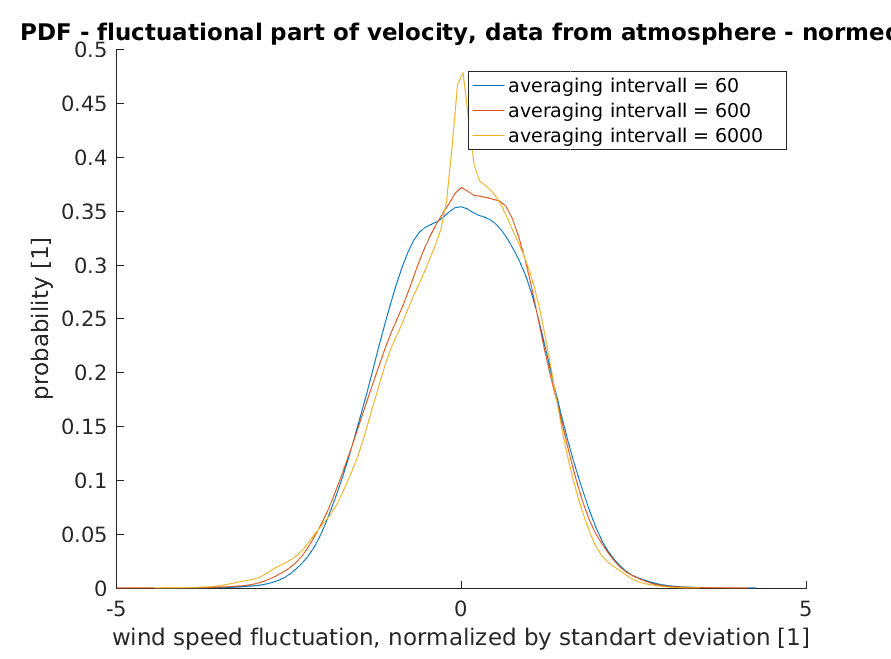
\includegraphics[width=1\linewidth]{figures/pdf_interval_comparison_atmosphere_normed.png}
  \caption{atmosphere, normed}
\end{subfigure}
\begin{subfigure}{0.5\textwidth}
  \centering
  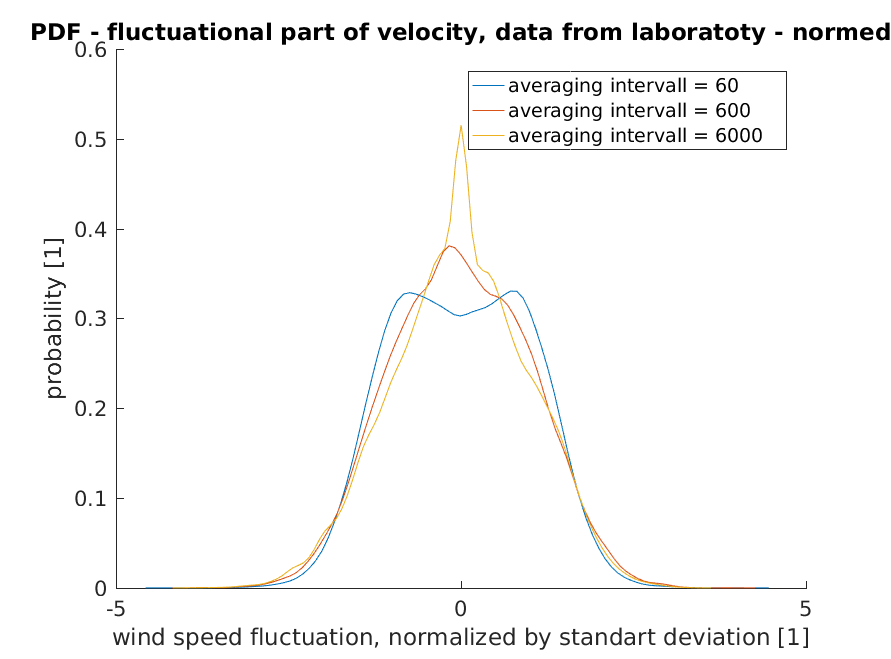
\includegraphics[width=1\linewidth]{figures/pdf_interval_comparison_fluc_labdata_normed.png}
  \caption{lab data, normed}
\end{subfigure}
\caption{Comparison of the normalized fluctuation for different averaging intervals}
\label{fig:pdf_fluc_normed}
\end{figure}
Both Figures show that there is a considerable difference in the fluctuation pattern for different averaging intervals. 10 minute intervals are often used in practice, however one has to consider the possible impact on the outcome, as shown in Figure\ref{fig:pdf_fluc} and Figure \ref{fig:pdf_fluc_normed}.
For completeness the basic characteristics have also been computed for different averaging intervals and are displayed in table~\ref{table:basic_char}.

\begin{table}[H]
\begin{center}
\begin{tabular}{c| c c c c}
\hline
Atmosphere &60&600&6000&complete\\
\hline
Mean &[m/s]&[m/s]&[m/s]&[m/s]\\
min&7.35&8.01&8.85&10.45\\
max&13.86&13.504&12.745&10.44\\
\hline
Magnitude of fluctuation &[m/s]&[m/s]&[m/s]&[m/s]\\

min&0.002&0.021&0.097&2.016\\
max&0.7144&1.1642&1.3711&2.016\\
\hline
Degree of Turbulence&$\%$&$\%$&$\%$&$\%$\\
min&2.129e-05&	0&	0&0.0185\\
max&0.006&	0.0109	&0.0103&0.0185\\
\hline
JFM data&60&600&6000&complete\\
\hline
Mean &[m/s]&[m/s]&[m/s]&[m/s]\\
min&1.035&	1.57&	2.07&	2.25\\
max&3.31&	2.81&	2,41&	2,25\\
\hline
Magnitude of fluctuation &[m/s]&[m/s]&[m/s]&[m/s]\\
min&1.56e-05&0.0164&0.10&0.1495\\
max&0.174&0.279&0.216&0.1495\\
\hline
Degree of Turbulence&$\%$&$\%$&$\%$&$\%$\\
min&1.20e-05&	0&	0	&0.0295\\
max&0.067&	0.071&0.041&	0.0295\\
\hline
\end{tabular}
\caption{Basic characteristics for different averaging intervals}
\label{table:basic_char}
\end{center}
\end{table}
\subsection{Conclusion}
Regarding the results of these comparisons the degree of turbulence in the JFM data (0.0295$\%$) is hhigher than the degree of turbulence in the measured atmospheric data (0.0185$\%$). This results seems reasonable because the JFM data was measured under fully developed turbulence conditions. Figure~\ref{fig:comparison_fluc} also shows that the fluctuation in the JFM dataset is more homogeneous and comes close to the idea of homogeneous turbulence. The variations in the atmospheric dataset might be due to changes of wind direction or day and night time conditions.

\begin{figure}[H]
\begin{subfigure}{0.5\textwidth}
  \centering
  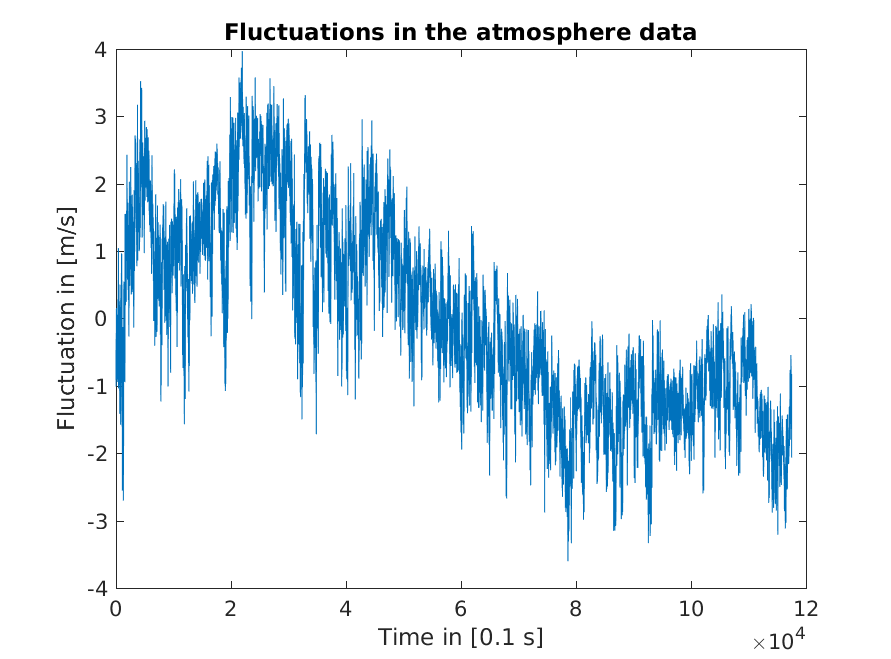
\includegraphics[width=1\linewidth]{figures/fluc_atmosphere.png}
  \caption{atmosphere}
\end{subfigure}
\begin{subfigure}{0.5\textwidth}
  \centering
  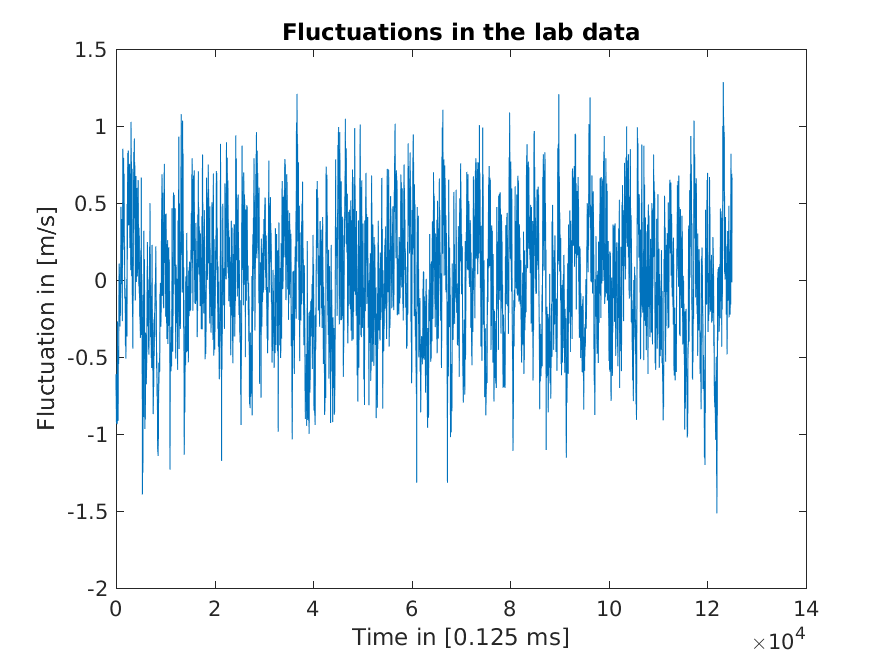
\includegraphics[width=1\linewidth]{figures/fluc_center.png}
  \caption{lab data}
\end{subfigure}
\caption{Comparison of the fluctuation in the different datasets}
\label{fig:comparison_fluc}
\end{figure}

As already mentioned the comparison of the different averaging intervals leads to very different results in their turbulent behaviour. But since only the lab results come close to homogeneous isotropic turbulence it is questionable to calculate the first and second order moment for the whole dataset. This outcome was already shown in Figure~\ref{fig:pdf_fluc}. In addition is has been shown that the wind speed distribution of the lab data can be fitted to a Gaussian distribution. That would also support the idea, that it is possible to describe the lab data only by it's first and second order moment. For the atmosphere dataset it's not possible to use a Gaussian fit, which means that further investigation is necessary in order to describe the dataset.

\section{Two-point quantities}

As see in the previous section one-point statistics are only able to give a good description of the dataset, if it is Gaussian distributed. In addition the shape of the signals sharing the same statistical properties cannot be distinguished from each other by one-point statistics. Therefore this section will deal with the characterization of correlations by two-point statistics. \cite{peinke2}
\subsection{Autocorrelation}
The basic statistical tools to analyse the correlations between two points in the time series of wind fluctuations are autocorrelation functions, wind increments and power spectrum analysis.
The autocorrelation is defined as
\begin{equation}
R_{uu}(\tau) = \frac{<u(t+\tau)\cdot u(t)>}{<u^{'2}>}
\end{equation}
The autocorrelation applies a time or spatial lag to the dataset and gives a and description of the degree of correlation. This is expressed in an autocorrelation coefficient on a scale from zero to one: Zero represents no correlation where one represents perfect correlation. It should be noted that the scale can also become negative which leads to a scale from minus one to zero. In this case minus one represents a perfect anti-correlation.
The wind increments are calculated by subtracting original data from a slightly shifted time series. This can be done for different lag intervals and will lead to dataset of increments depended on the time lag. Increments are defined as
\begin{equation}
\Delta(ut,\tau) = u (t+\tau) - u (t)
\end{equation}
Lastly it was mentioned that it is also possible to perform a power spectrum analysis which is similar to the autocorrelation approach. The power spectrum analysis can be formed by using a Fast Fourier Transformation of the autocorrelation, which will be shown in the following chapter. The different approach to calculate the power spectrum, which was used at first, is to perform the FFT of the measured signal. The spectral energy density shows therefore how much energy is related to a certain frequency interval.
\subsection{Power spectrum analysis}
As mentioned above the energy density spectrum can be used to describe, the energy distribution in the dataset. It also shows how much energy is contained by different frequencies. Kolmogorov (1941) stated turbulent motions span a wide range of scales ranging from the macroscale, at which energy is supplied to the microscale at which energy is dissipated by viscosity. The energy is passed from the macroscale to the microscale, which is known as energy cascade. If the state of turbulence is statistically steady (which we will assume later, by applying Taylor's Frozen Turbulence) the rate of energy transfer from one scale to another should be the same. \cite{cushman} The following Figures shows the power spectrum for both datasets. It was calculated by performing a FFT on the dataset and then squaring the outcome. 
\begin{figure}[H]
\begin{subfigure}{0.5\textwidth}
  \centering
  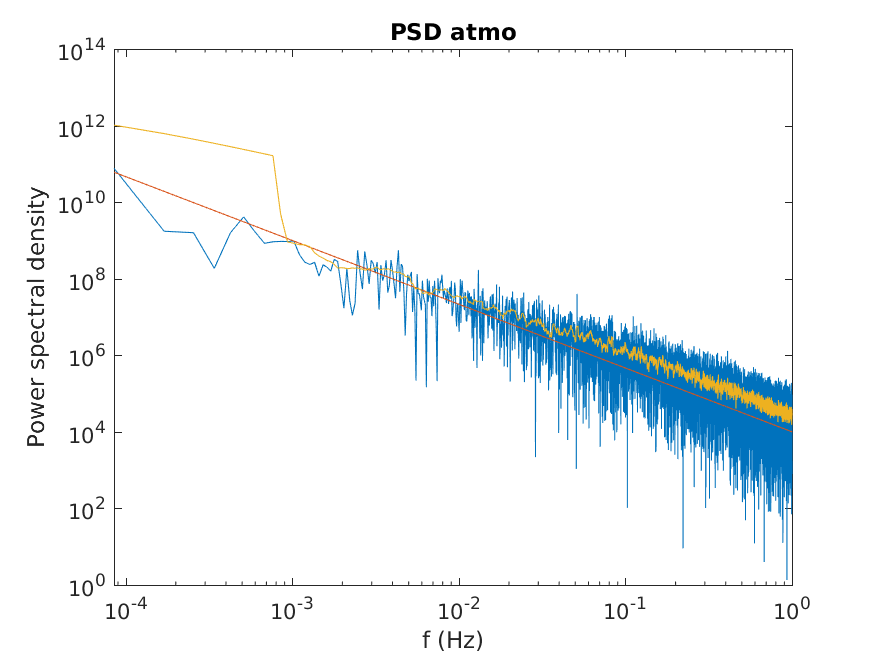
\includegraphics[width=1\linewidth]{figures/power_spectrum_atmo_smooth.png}
  \caption{atmosphere}
\end{subfigure}
\begin{subfigure}{0.5\textwidth}
  \centering
  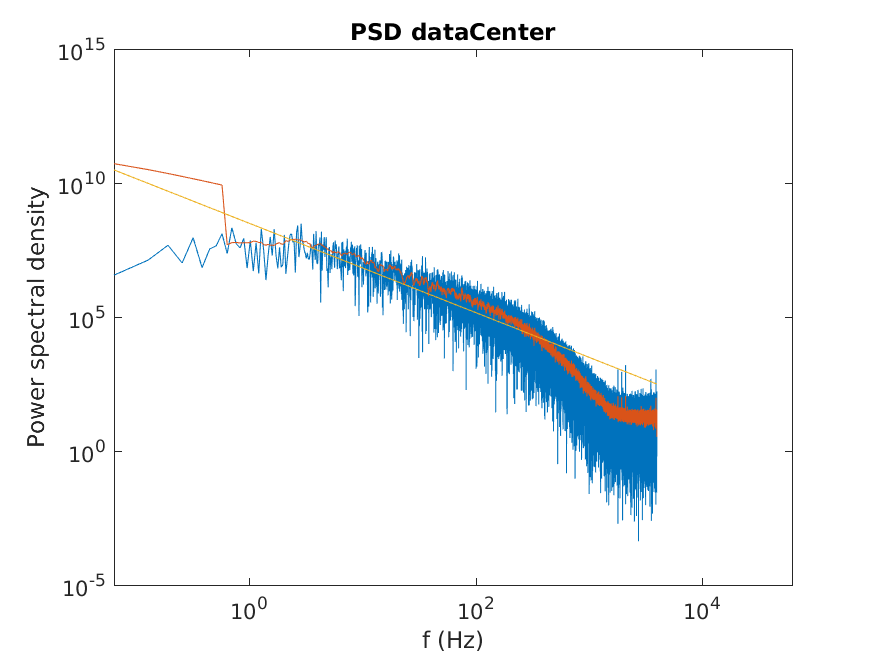
\includegraphics[width=1\linewidth]{figures/power_spectrum_center_smooth.png}
  \caption{lab data}
\end{subfigure}
\caption{Comparison of the power spectral density}
\label{fig:comparison_fluc}
\end{figure}
Based on the Kolmogorov41 which was discussed above a fit was added to the Figures, called -5/3 law. This method assumes an equally distributed dissipation rate over all scales within the inertial sub-range. If plotted logarithmic it has a linear shape.
The equation based on this theory is shown below:
\begin{equation}
E(k) = C * \epsilon_0^{2/3}k^{-5/3}
\end{equation}
In order to reduce the noise in the spectrum the curve was smoothed. This allows a better visualisation of the curves slope. The smoothing can be performed by simple using the command $smooth()$ in Matlab.

\subsection{Fourier transform of the autocorrelation}
In the introduction it was discussed that there are different possibilities to derive the power spectrum. Figure~\ref{fig:comparison_fluc} was calculated by performing a FFT on  the dataset and the squaring the outcome. The second method which is now presented is called Wiener-Khinchin theorem. It states that the Fourier transformation of the autocorrelation function of a 'wide sense-stationary random process' can be used as a parametric method to estimate the power spectrum. \cite{chatfield}(It should be noted here, that there are a lot of other different ways to compute the PSD). The aim of this task was not, to make a comparison between these two methods, but to show that they are numerically equal. In the following code snippet it is shown how the power spectrum was computed:
\begin{lstlisting}
%atmosphere
autocorr_atmo  = xcorr(atmosphere,atmosphere,length(f_atmo));
fft_auto_corr_atmo = fft(autocorr_atmo);
fft_auto_corr_atmo = abs(fft_auto_corr_atmo);
fft_auto_corr_atmo = fft_auto_corr_atmo(1:length(atmosphere)/2+1);
\end{lstlisting}
To compare the two different methods, the two calculated power spectra are plotted in the same Figure. The outcome for both datasets is shown in Figure~\ref{fig:comparison_power}.

\begin{figure}[H]
\begin{subfigure}{0.5\textwidth}
  \centering
  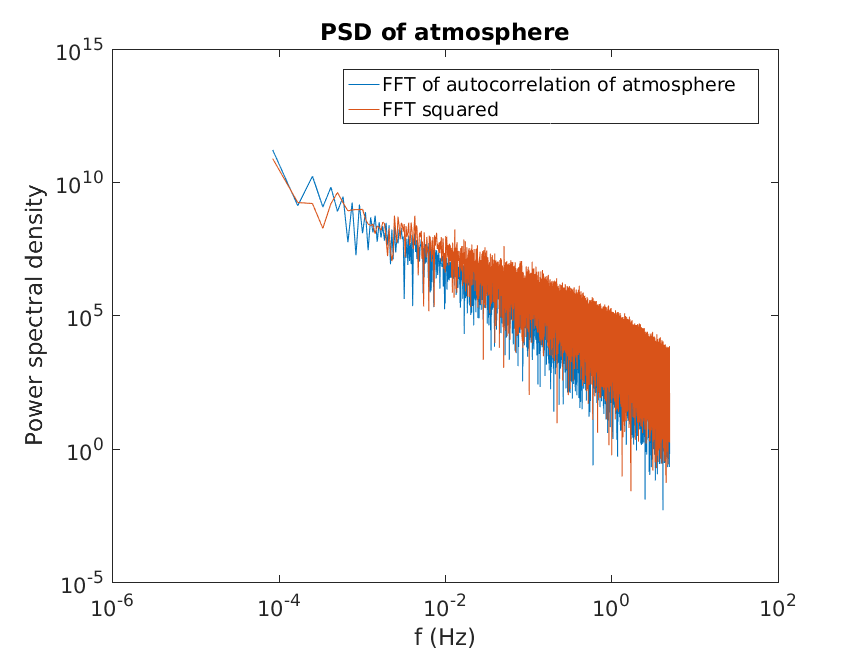
\includegraphics[width=1\linewidth]{figures/atmo_numerically_equal.png}
  \caption{atmosphere}
\end{subfigure}
\begin{subfigure}{0.5\textwidth}
  \centering
  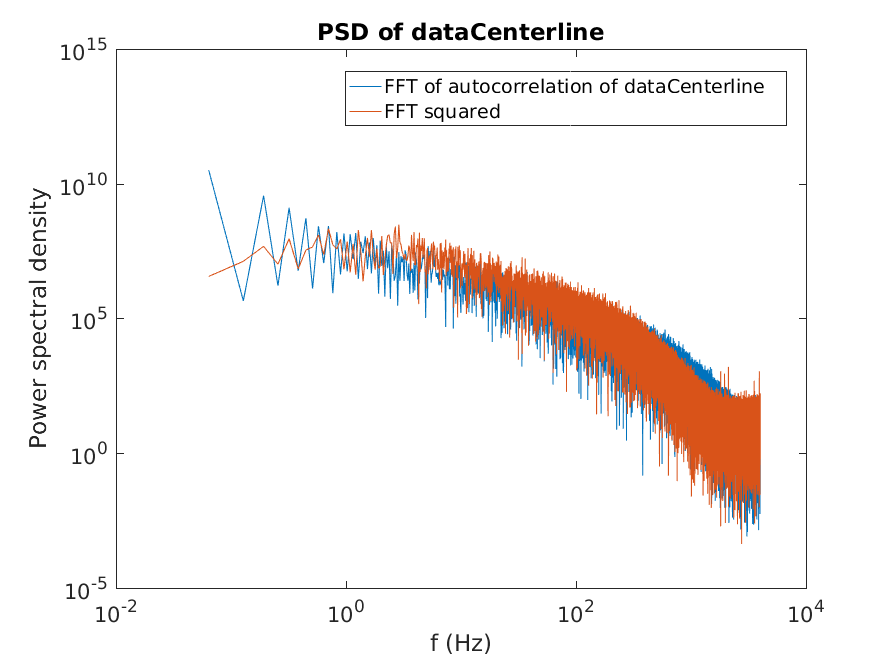
\includegraphics[width=1\linewidth]{figures/center_numerically_equal.png}
  \caption{lab data}
\end{subfigure}
\caption{Comparison of different ways to derive the power spectrum}
\label{fig:comparison_power}
\end{figure}

The Fourier transformation of the autocorrelation function, displayed in orange, produces similar results for both datasets. There are only slight differences in total. For the PSD of the atmosphere dataset a small shift can be noticed.

\subsection{Joint Probability Distribution}
The autocorrelation function of the fluctuation can be expressed by the joint probability density, which is defined by:

\begin{equation}
<v^{'}(t)v^{'}(t+\tau)> = \int_{-\infty}^{+\infty}\int_{-\infty}^{+\infty} v^{'}(t)v^{'}(t+\tau)p(v^{'}(t),v^{'}(t+\tau))dv^{'}(t)dv^{'}(t+\tau)
\end{equation}
\begin{figure}[H]
\begin{subfigure}{0.5\textwidth}
  \centering
  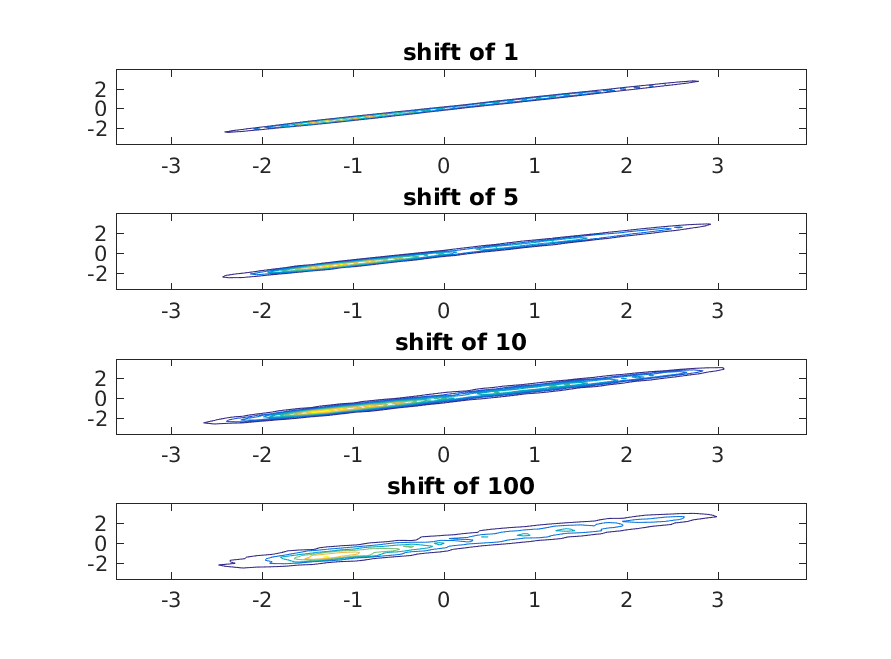
\includegraphics[width=1\linewidth]{figures/jpdf_atmo.png}
  \caption{atmosphere}
\end{subfigure}
\begin{subfigure}{0.5\textwidth}
  \centering
  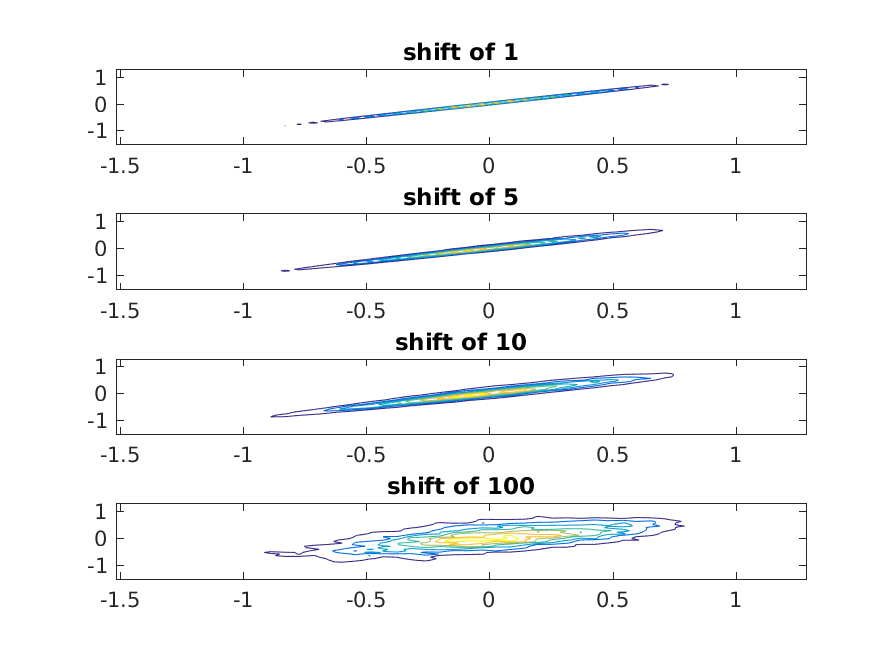
\includegraphics[width=1\linewidth]{figures/jpdf_center.png}
  \caption{lab data}
\end{subfigure}
\caption{Comparison of Joint Probability Density Functions of the fluctuation for both datasets}
\label{fig:comparison_jpdf}
\end{figure}
Figure~\ref{fig:comparison_jpdf} shows the correlation for different time lags in the dataset. For the visualisation the $contour()$ function in Matlab was used. Both Figures show a good correlation for a shift of 1 timestep. With increasing time shift the correlation is getting smaller and smaller. This outcome was expected since the fluctuation should be more dependent on smaller timelags than bigger timelags. As already mentioned the lab data displays nearly perfect isotropic homogeneous turbulence. Therefore the Joint PDF plot in Figure~\ref{fig:comparison_jpdf} (b) represents what is theoretically predicted.
\subsection{Length scales}
\subsubsection{Integral length}
In this report the energy cascade was already discussed. Energy is supplied at the macroscale and passed on until it dissipates in at the microscale. The Integral scale marks the size of the largest eddies occurring in the turbulent flow. The largest eddies in the flow account for most of the transport of momentum and energy and their size is only constrained by the physical boundaries of the flow. There are different ways to calculate the integral length. In this report Taylor's Hypothesis was used. It states that vortices or turbulence patterns change so slowly that they can be considered to be frozen while passing the sensor. Therefore the diameter of a structure can be calculated. That means that a time signal can be transformed into a scale signal by means of Taylor's hypothesis. \cite{tutorial} With this assumption the integral length was calculated from the autocorrelation function of the energy spectrum, whereas the autocorrelation function was integrated from zero to the first zero crossing. The equation used for this approach is give below.
\begin{equation}
L = \frac{1}{<v^2(x)>}\int_{0}^{+\infty}<v(x)v(x+r)>dr
\end{equation}
As already mentioned, this only one way to derive the integral length. 
\subsubsection{Taylor length}
The Taylor micro scale is the intermediate length scale at which fluid viscosity affects the dynamics of the turbulent eddies in the flow. Length scales larger than Taylor's microscale are not strongly affected by viscosity. The region between the Integral length and Taylor's microscale is called inertia range. To estimate the Taylor microscale $\lambda$ the following equation was used:

\begin{equation}
\lambda^2 = \frac{<u'^2>}{(\frac{\partial u'}{\partial x})^2}
\end{equation}


\subsubsection{Kolmogorov length}
The smallest length scale at which energy is dissipated into heat is called Kolmogorov length. It represents the smallest eddies in the flow. For the further calculation two equations are needed:

\begin{equation}
\eta = (\frac{\nu^3}{\epsilon})^{0.25}
\end{equation}
\begin{equation}
\epsilon = 15 \cdot \nu * \frac{<u'^2>}{\lambda^2}
\end{equation}

\subsubsection{Results}
\begin{table}[H]
\begin{center}
\begin{tabular}{c c c}
\hline
Length scales & atmosphere & JFM\\
\hline
Integral length scale & 1.70 km &59 mm\\
Taylor's microscale & 0.1420 m & 0.48 mm\\
Kolmogorov length scale & 4.5mm & 0.25 mm\\
\hline
\end{tabular}
\caption{Turbulent Length Scale for both datasets}
\label{table:length_scales}
\end{center}
\end{table}
Table~\ref{table:length_scales} shows the problem with Taylor's hypothesis. The measured frequency of 10 Hz for the atmosphere dataset might be to low to assume frozen turbulence. However one can clearly see, especially for the JFM dataset, the difference in eddy size/length scale.
\subsection{Velocity increments and structure functions}
Fine scale structures of turbulence are evaluated by the introduction of velocity increments. 
\begin{equation}
v_x(r,t) = u(x+r,t)-u(x,t)
\end{equation}
The so called structure functions are by definition time moments of the velocity increments. \cite{peinke} The application of the momentum approach is defined as:
\begin{equation}
S^n(\tau) = <(\delta_{\tau}v(t))^n> = <v(t+\tau)-v(t))^n>
\end{equation}
\subsubsection{Velocity increments}
The wind speed increments consider the difference between two points of a turbulent eddy with a fixed time or spatial lag. Analogous two the approach before the spatial time lag is considered in this report. It was asked to check, how the magnitude of the fluctuations change with an increasing spatial lag of $r = 2^m$. In the following Figure the velocity increments for both datasets are shown for $r = 2^1, 2^2, 2^5$.
\begin{figure}[H]
\begin{subfigure}{0.5\textwidth}
  \centering
  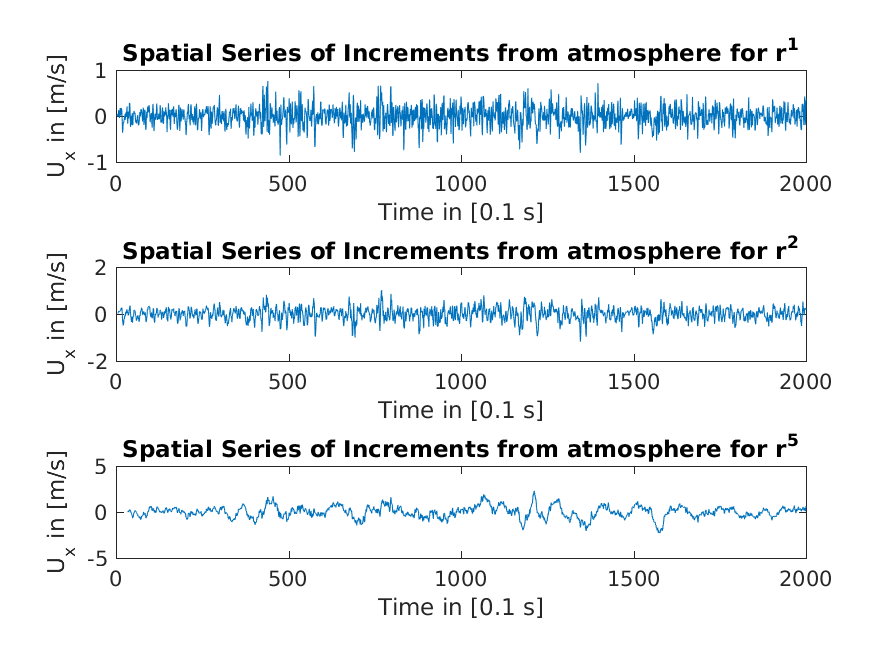
\includegraphics[width=1\linewidth]{figures/increments_array_atmo.png}
  \caption{atmosphere}
\end{subfigure}
\begin{subfigure}{0.5\textwidth}
  \centering
  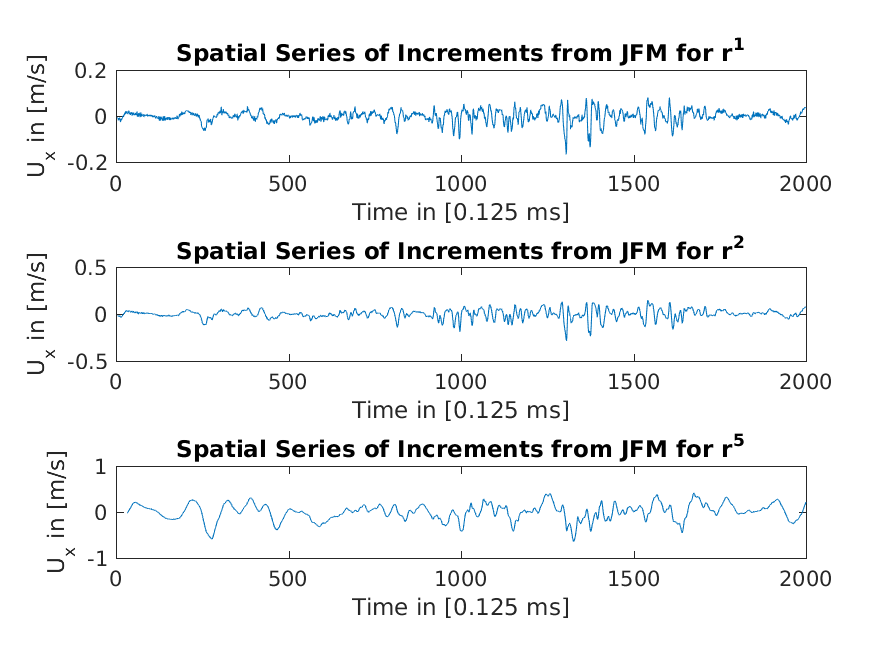
\includegraphics[width=1\linewidth]{figures/increments_array_center.png}
  \caption{lab data}
\end{subfigure}
\caption{Comparison of different velocity increments for both datasets}
\label{fig:comparison_velo_incr}
\end{figure}
Figure~\ref{fig:comparison_velo_incr} shows the increasing fluctuation with an increasing spatial lag $r^m$. A method to describe the statistics of the wind speed increments is to calculate the PDF functions for different lags. This method is analogous to the method used before. Taking into account that the wind speed increments distribution can be fully described if they are Gaussian-distributed. When this condition is not given, higher order moments have to be calculated to describe the PDF function. In Figure~\ref{fig:comparison_pdf_incr} the PDF functions for different lags are displayed for both datasets. 
\begin{figure}[H]
\begin{subfigure}{0.5\textwidth}
  \centering
  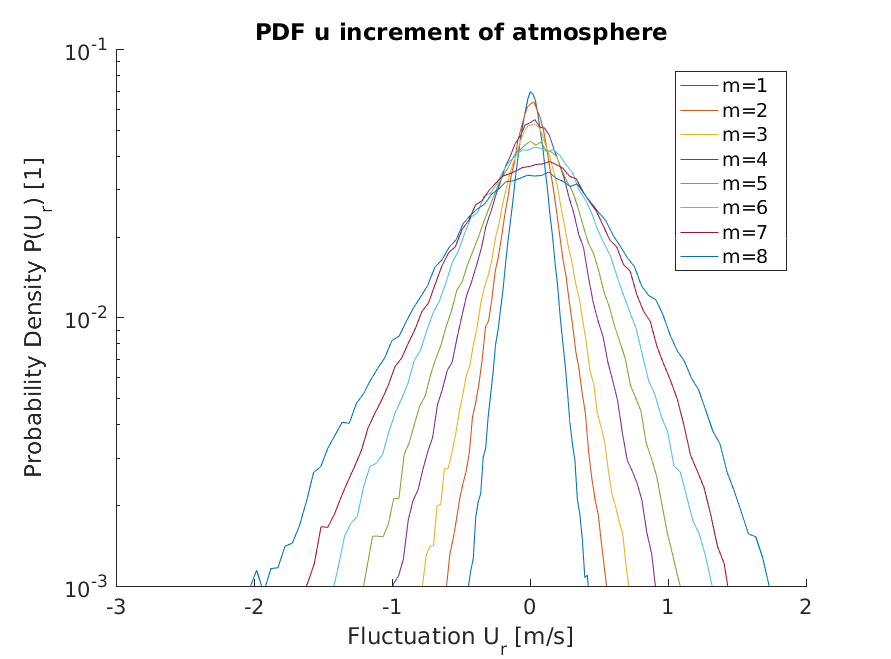
\includegraphics[width=1\linewidth]{figures/pdf_increments_atmo.png}
  \caption{atmosphere}
\end{subfigure}
\begin{subfigure}{0.5\textwidth}
  \centering
  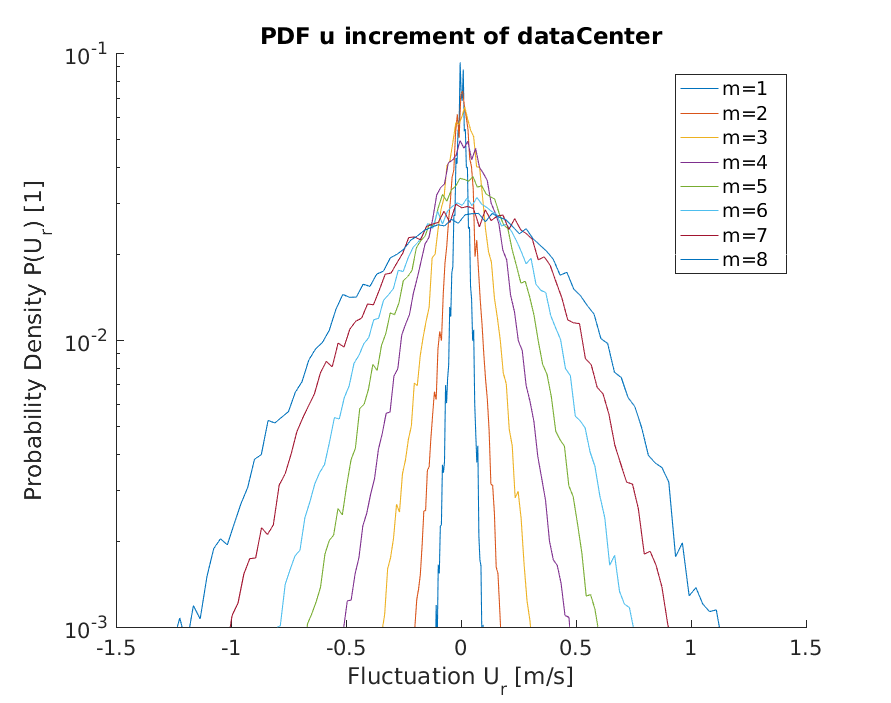
\includegraphics[width=1\linewidth]{figures/pdf_increments_center.png}
  \caption{lab data}
\end{subfigure}
\caption{Comparison of PDF functions of velocity increments for both datasets}
\label{fig:comparison_pdf_incr}
\end{figure}
The Figure shows that the fluctuation distribution changes for different lags. In order to show, what this means for the characterisation of the PDF function, Figure~\ref{fig:comparison_pdf_incr_18} shows how good a Gaussian fit is applicable.

\begin{figure}[H]
\begin{subfigure}{0.5\textwidth}
  \centering
  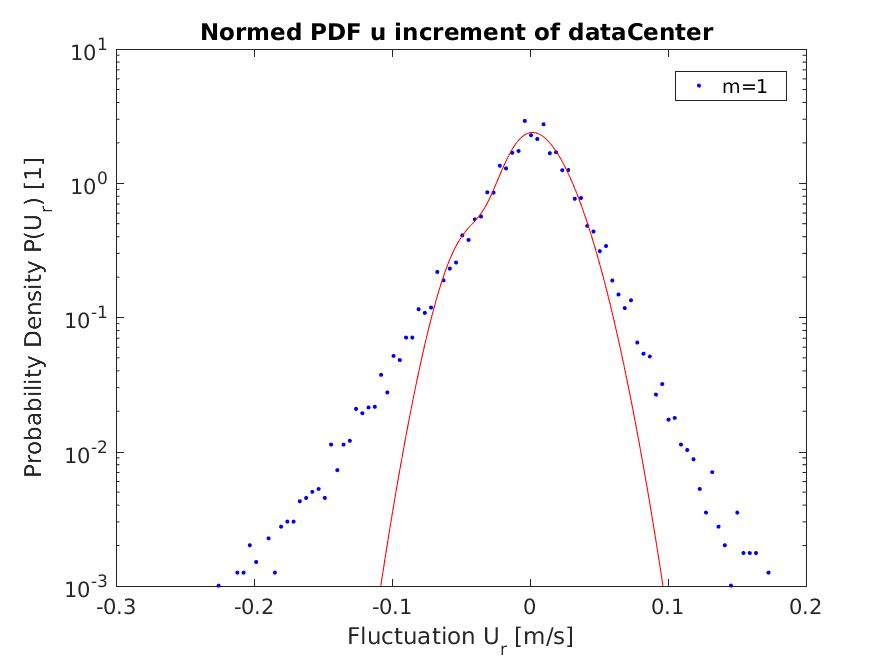
\includegraphics[width=1\linewidth]{figures/pdf_increments_center_normed_1.png}
  \caption{lab data with $r = 2^1$}
\end{subfigure}
\begin{subfigure}{0.5\textwidth}
  \centering
  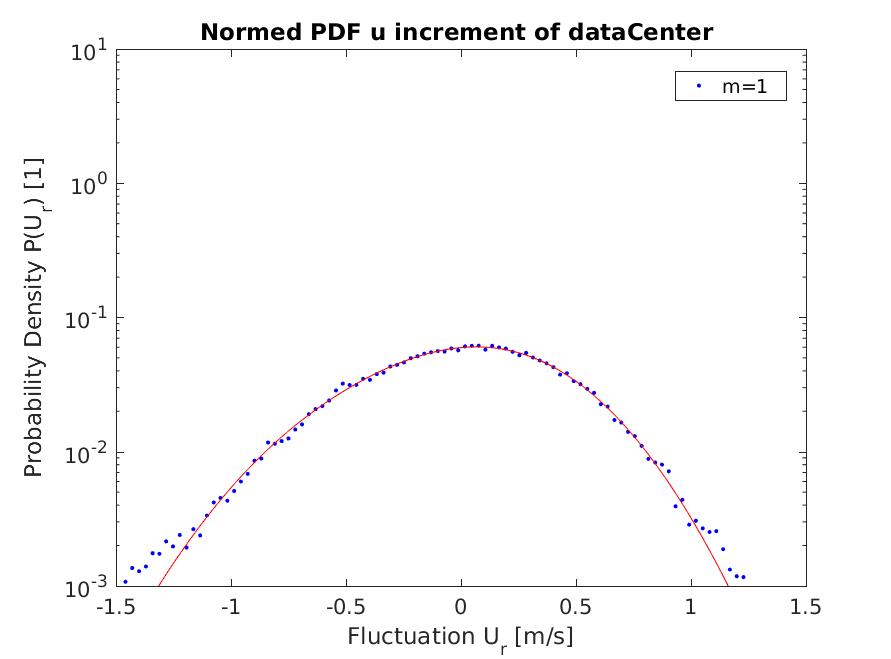
\includegraphics[width=1\linewidth]{figures/pdf_increments_center_normed_8.png}
  \caption{lab data with $r = 2^8$}
\end{subfigure}
\caption{Comparison of Gaussian fit for different time lags}
\label{fig:comparison_pdf_incr_18}
\end{figure}

The Figure shows, that for smaller lags a Gaussian fit is not applicable. This is outcome was expected since the joint PDF function have already shown that for greater lags the dataset becomes uncorrelated. However both Increment PDF's show a good fit for the region around the mean. Higher fluctuations follow a different distribution and cannot described by the Gaussian distribution. (Regarding smaller lags)
A direct comparison between the two datasets is only possible by regarding the normalized PDFs in Figure~\ref{fig:comparison_pdf_incr_normed}.

\begin{figure}[H]
\begin{subfigure}{0.5\textwidth}
  \centering
  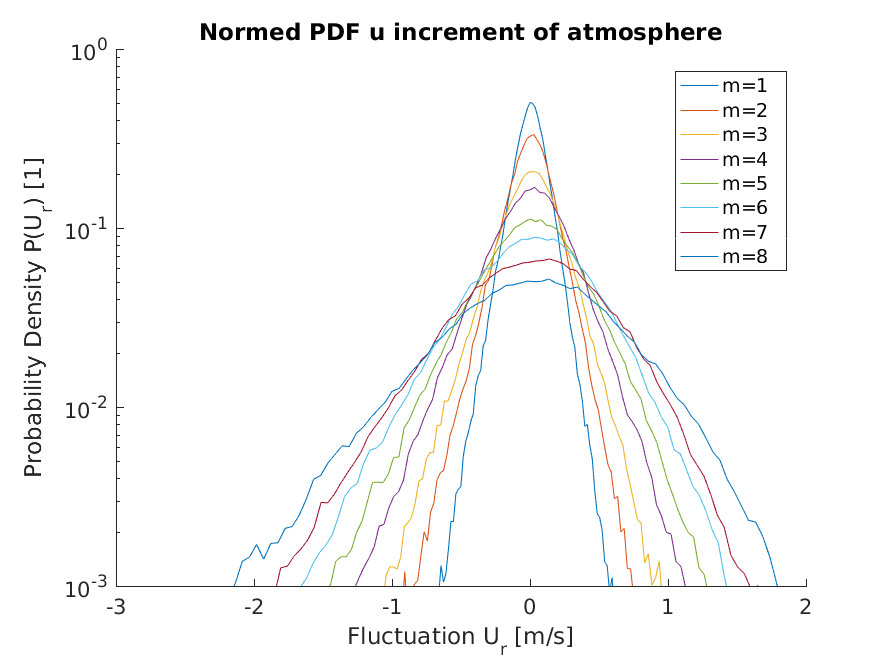
\includegraphics[width=1\linewidth]{figures/pdf_increments_atmo_normed.png}
  \caption{atmosphere}
\end{subfigure}
\begin{subfigure}{0.5\textwidth}
  \centering
  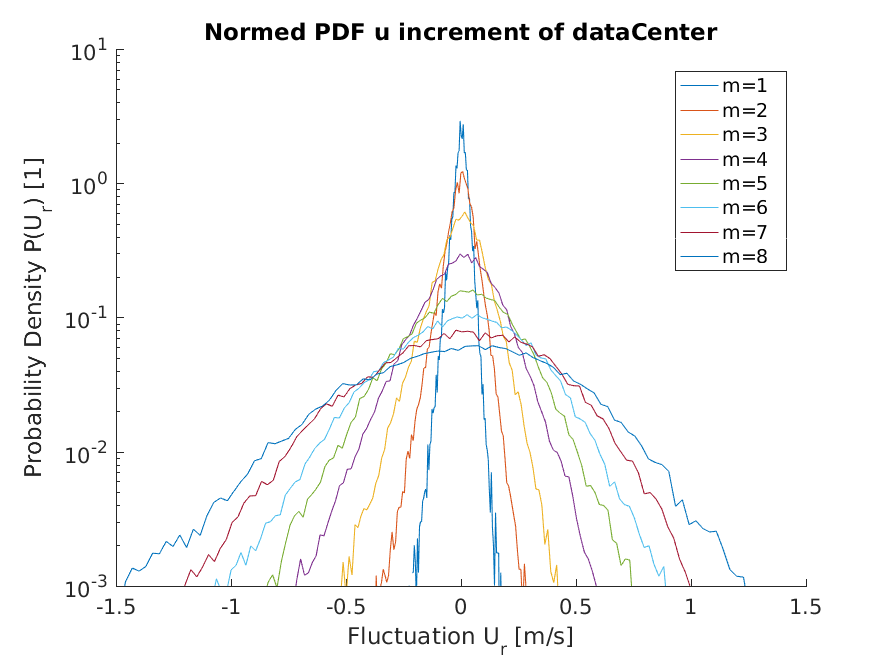
\includegraphics[width=1\linewidth]{figures/pdf_increments_center_normed.png}
  \caption{lab data}
\end{subfigure}
\caption{Comparison of Normed PDF functions of velocity increments for both datasets}
\label{fig:comparison_pdf_incr_normed}
\end{figure}

It can be seen that the lab dataset compared to the atmosphere dataset has a higher peak for smaller time lag and is less Gaussian distributed. Still, the lab data converges faster to the Gaussian distribution. This might be due to the fact that the inertia sub-range is smaller in the lab dataset. That means that the integral length scale, which is considered as a limit for the maximum lag size, is reached faster with increasing lag distance.
\subsubsection{Structure functions}
Structure functions are used to describe the increment statistics. Again as already introduced, structure functions are defined by:
\begin{equation}
S^n(\tau) = <(\delta_{\tau}v(t))^n> = <v(t+\tau)-v(t))^n>
\end{equation}
That means the structure functions are defined by their order of n. Therefore they show, how the increments change with the order n as a function of lag distance r. The calculation of the structure function was by simply raising the increments to the power of n and using and ensemble mean. In the following Figure the structure functions S(n,r) where calculated and plotted against the lag distance r. Each structure function represents a different moment of order n. Some structure functions are related to special turbulent characteristics. The second order moment is related to the autocorrelation. The third order moments are related to the energy transfer of the turbulence. 

Kolmogorov presented in 1941 an equation with describes the structure functions as a function of energy dissipation rate, lag and the moment order within the inertial sub-range. 

\begin{equation}
S_n(r) \propto (\epsilon_0 \cdot r)^{n/3}
\end{equation}
The equation shows that the structure function plotted in a logarithmic scale should have a linear slope. For example the structure function of the third order moment has a slope of 1.

\begin{figure}[H]
\begin{subfigure}{0.5\textwidth}
  \centering
  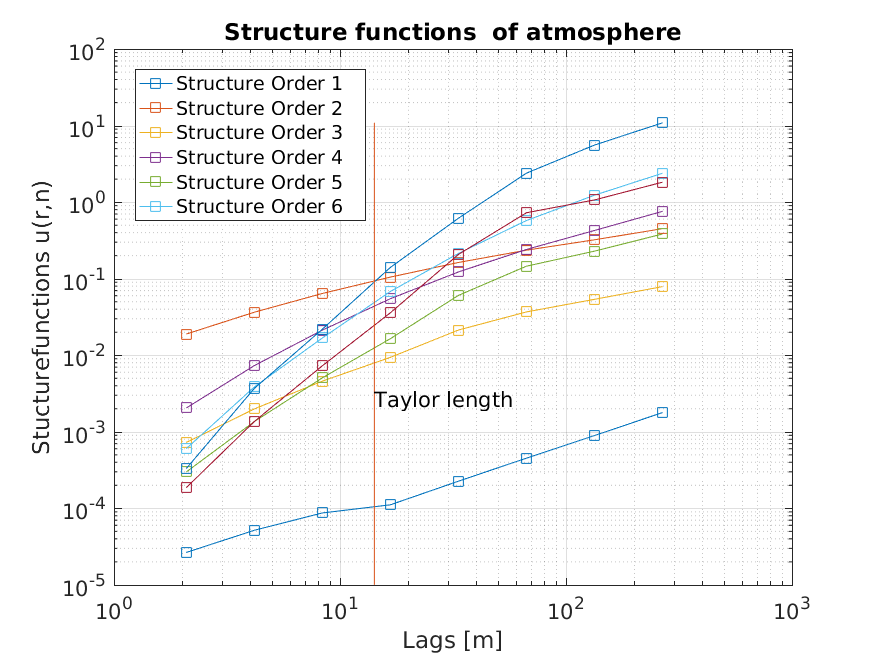
\includegraphics[width=1\linewidth]{figures/structure_atmo.png}
  \caption{atmosphere}
\end{subfigure}
\begin{subfigure}{0.5\textwidth}
  \centering
  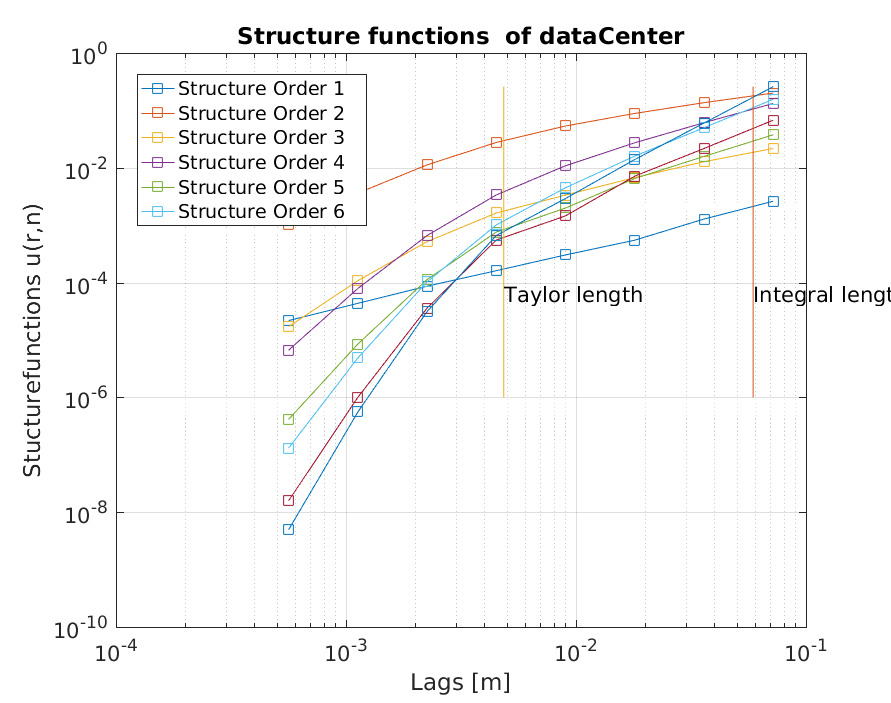
\includegraphics[width=1\linewidth]{figures/structure_center.png}
  \caption{lab data}
\end{subfigure}
\caption{Comparison of structure functions for both datasets}
\label{fig:comparison_pdf_incr_normed}
\end{figure}
It can be seen that the assumption of a linear slope holds true for the lab data, whereas the atmosphere dataset does not always follow a linear shape. The deviation from the Kolmogorov41 prediction is due to the intermittency occuring within the turbulent flow. The basic assumption of the Kolmogorov41 prediction is, that the statistical properties of the velocity field are locally homogeneous and isotropic and that there exists a constant energy cascade from large to small scales. \cite{benzi}
In order to compare the deviation from the Kolmogorov41 prediction the slope was calculated for the inertia sub-range and plotted for increasing order of moments n. The same approach was done for the Kolmogorov41 prediction and also the Kolmogorov62. Kolmogorov62 takes intermittency into account is defined as:
\begin{equation}
\theta_n = \frac{n}{3} - \frac{n(n-3)}{2}\delta
\end{equation}
The parameter $\delta$ describes the correction of the Kolmogorov41 law and was experimentally estimated. As already mentioned with this approach, we can only discuss results for the inertia sub-range. However R. Benzi proposed a method called extended self-similarity which exceeds the inertial sub-range. Extended self-similarity means therefore, that each structure function should have approximately the same shape. That is why R. Benzi decided to plot the structure functions against a reference structure function to compare deviations of the shape. Often the structure function of the 3rd order is used. However this is not necessary. Figure~\ref{fig:comparison_sr} shows the application of this method.
\begin{figure}[H]
\begin{subfigure}{0.5\textwidth}
  \centering
  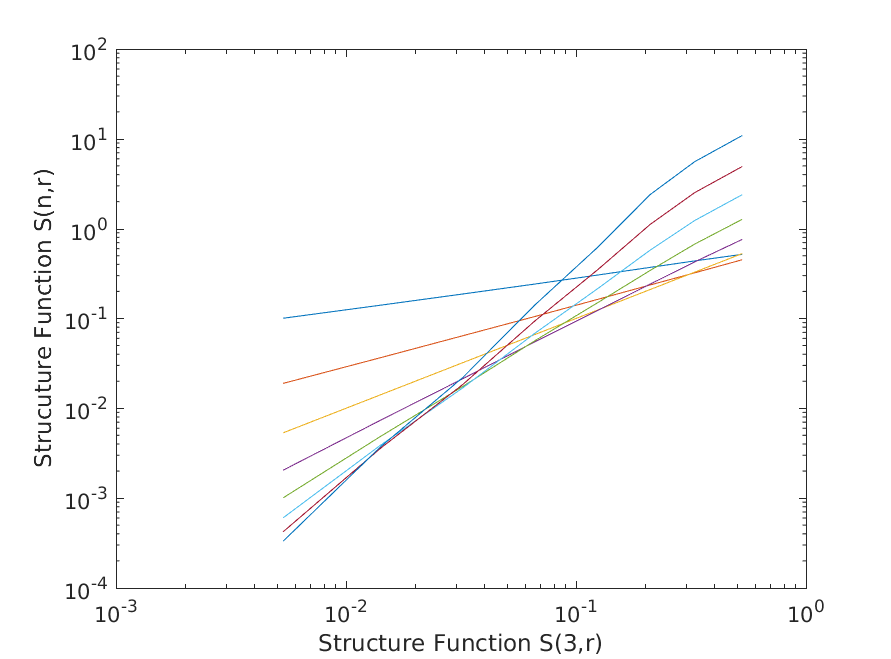
\includegraphics[width=1\linewidth]{figures/ess_compare_atmo.png}
  \caption{atmosphere}
\end{subfigure}
\begin{subfigure}{0.5\textwidth}
  \centering
  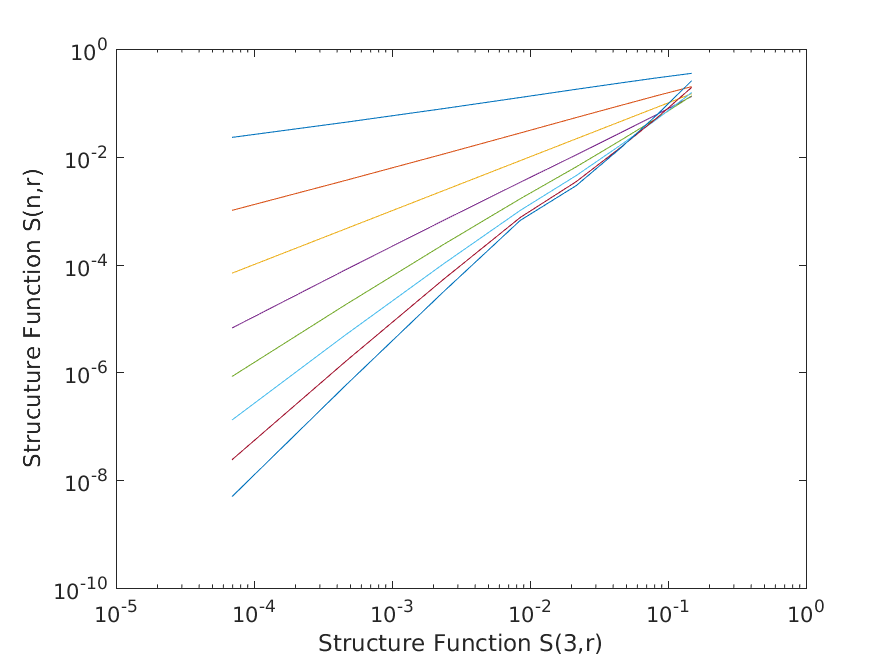
\includegraphics[width=1\linewidth]{figures/ess_compare_center.png}
  \caption{lab data}
\end{subfigure}
\caption{Structure functions plotted against S(3,r)}
\label{fig:comparison_sr}
\end{figure}
It can be seen, that there is a bigger range of self similarity in the lab dataset. For the atmosphere dataset the ESS is not as clear as in the JFM dataset, but the structure functions mostly have a linear shape. 
In order to get an idea how the different methods are related to each other, they were plotted in Figure~\ref{fig:comparison_ess}
\begin{figure}[H]
\begin{subfigure}{0.5\textwidth}
  \centering
  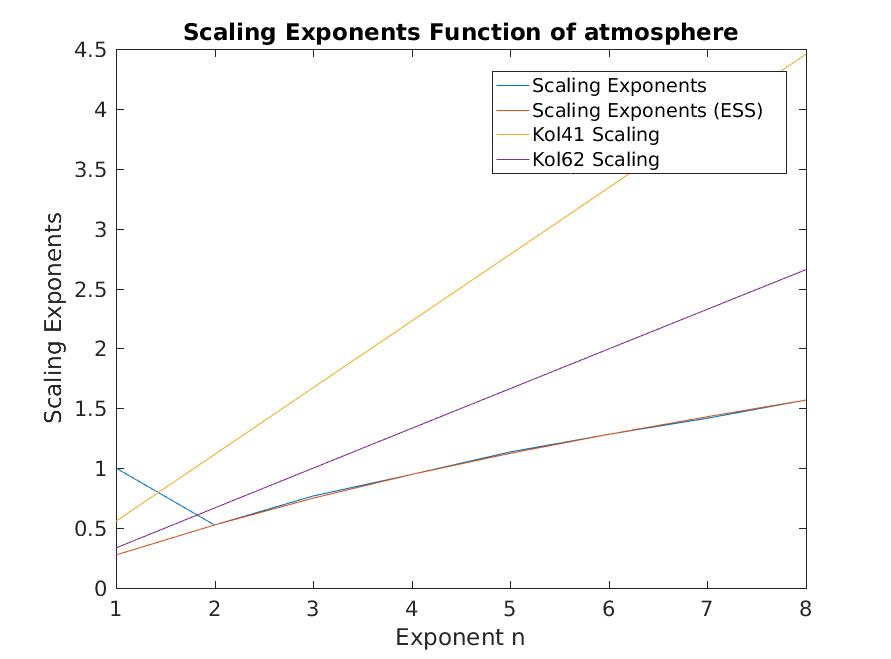
\includegraphics[width=1\linewidth]{figures/scale_compare_atmo.png}
  \caption{atmosphere}
\end{subfigure}
\begin{subfigure}{0.5\textwidth}
  \centering
  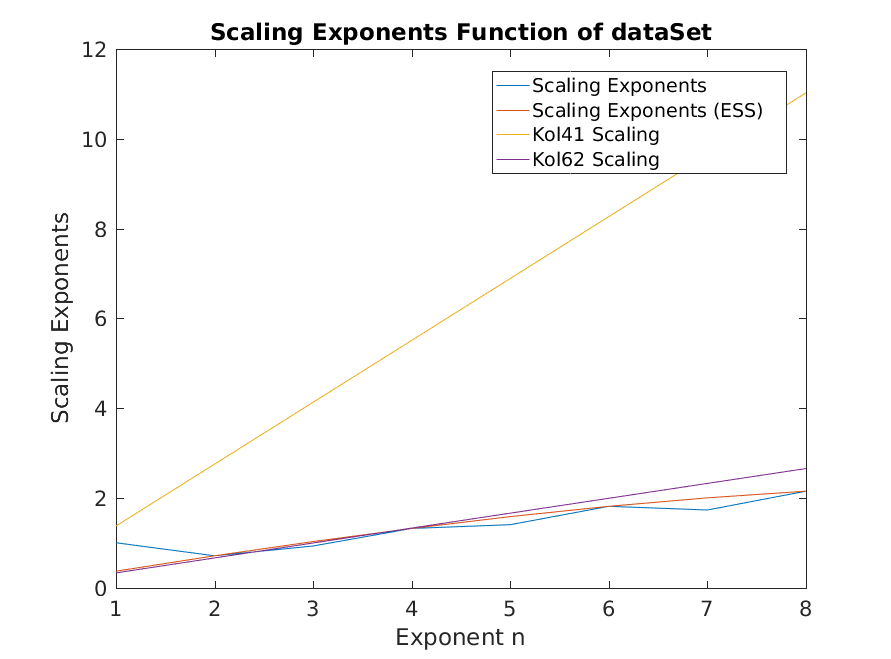
\includegraphics[width=1\linewidth]{figures/scale_compare_center.png}
  \caption{lab data}
\end{subfigure}
\caption{Comparison of Scaling Exponents both datasets}
\label{fig:comparison_ess}
\end{figure}
The scaling exponent function of the atmosphere dataset deviates very strongly from the Kolmogorov41 prediction. It also deviates very strongly from the Kolmogorov62 prediction, which takes intermittency into account. This shows that scaling methods for ideal turbulence cannot be easily transferred on atmospheric measurements. However there is a short range for exponents n from 1-3, where the deviation to the Kolmogorov62 is still acceptable. But this changes quickly for greater exponents.
The lab dataset shows a very good fit for the Kolmogorv62 prediction. This holds true for greater exponents and therefore exceed Kolmogorovs prediction for self-similarity. This leads to a wider range of scales than as summed where self-similarity can be identified. \\
It has been already shown, that for the atmosphere dataset ideal turbulent can not be assumed. The measurement system is influenced by weather conditions and is limited in the spatial resolution. The anemometer might have missed small eddies. In general it should be questioned whether an anemometer is able to measure turbulence behaviour. That leads to the question whether the dataset can be used for turbulence investigations.
\section{N-Point quantities}
The standard approach to analyse small scale turbulence is based two-point correlations and their dependence on the distance between the two points. A central point of this approach is to use velocity increments. Since most of the turbulent flows are complex 3-dimensional systems it might be necessary to perform multi-point correlations. This approach is called n-point statistics. These n-point quantities can be displayed in Joint PDFs. The Joint PDFs can be derived by calculating the Conditional PDFs. In this chapter the conditioned probabilities for $p(u_r | u_{r'})$ are further examined. It should be noted that the applied lag $r_1$ has to be smaller than $r_2$ in order to fulfil the condition for a Markov's process. If these two quantities are known, no higher scales have to be taken into account. The conditional PDF displays the probability density of the wind speed increment occurring, when a different wind speed increment has already occurred.\cite{npoint} The outcome is shown in Figure~\ref{fig:npoint_atmo} and Figure~\ref{fig:npoint_center}.
\begin{figure}[H]
  \centering
  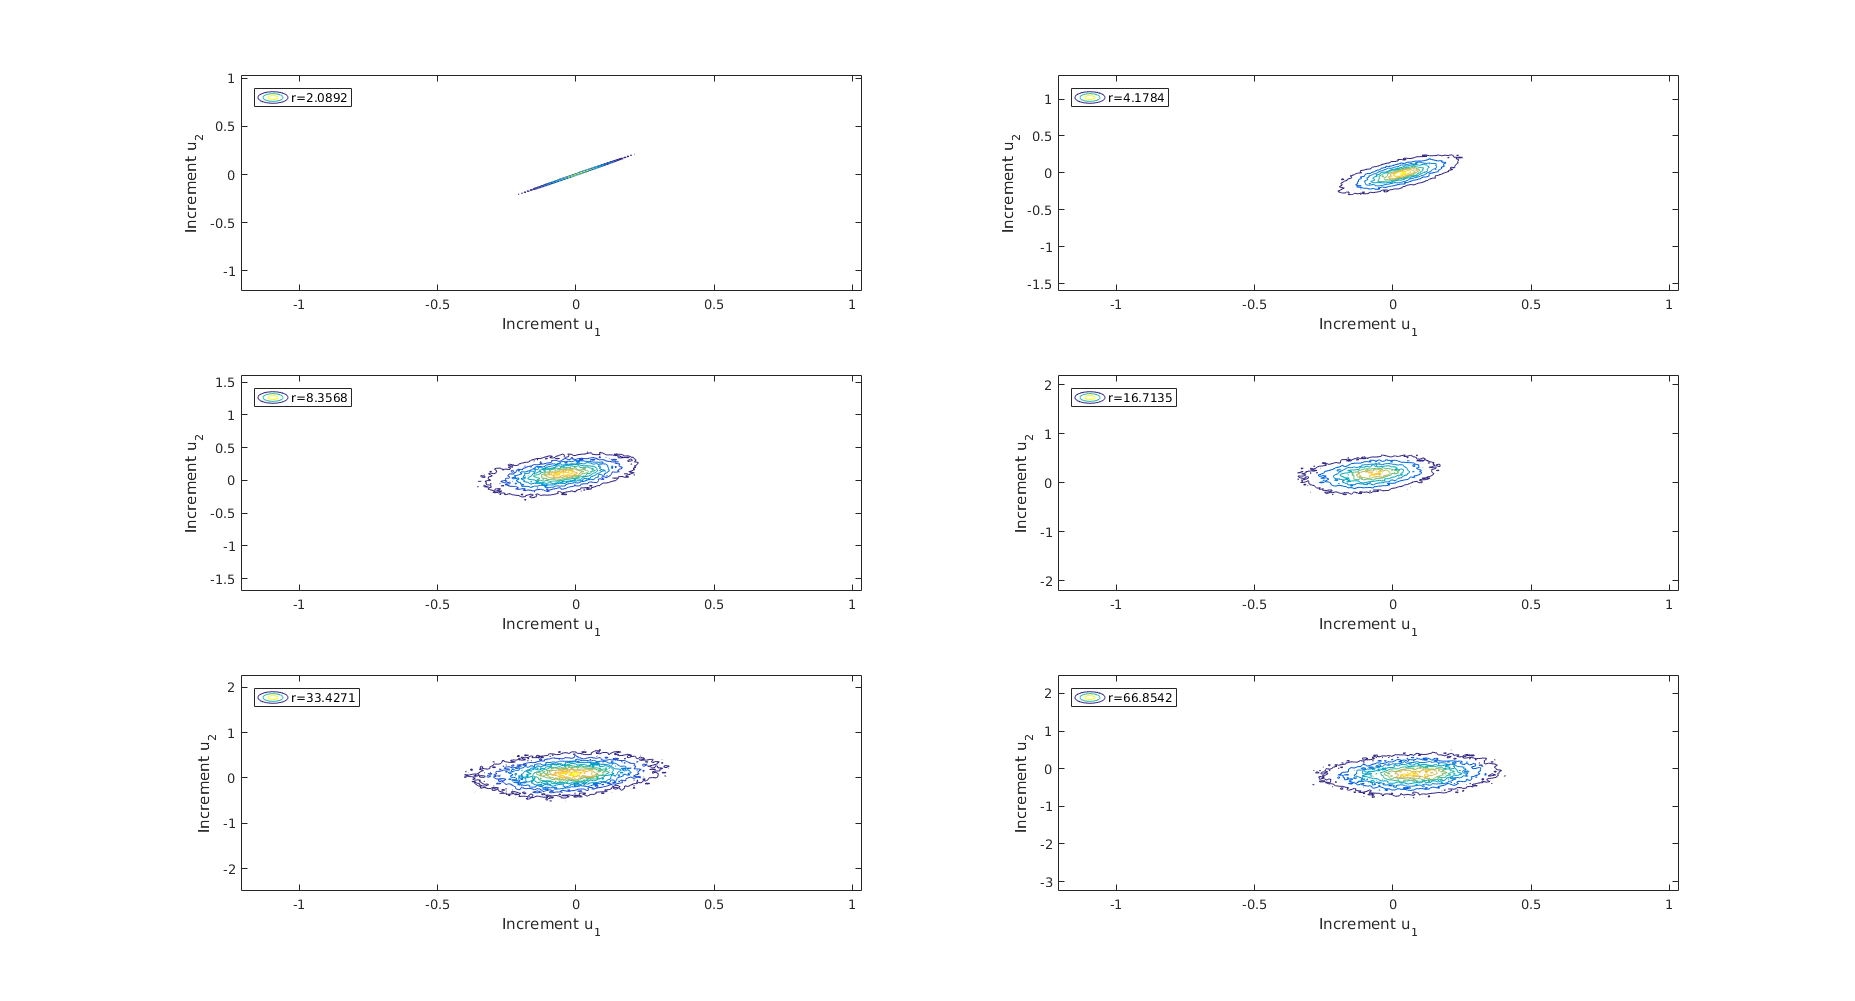
\includegraphics[width=1\linewidth]{figures/atmo_npoint.png}
\caption{Conditional PDF of atmosphere with increasing time lag}
\label{fig:npoint_atmo}
\end{figure}
\begin{figure}[H]
  \centering
  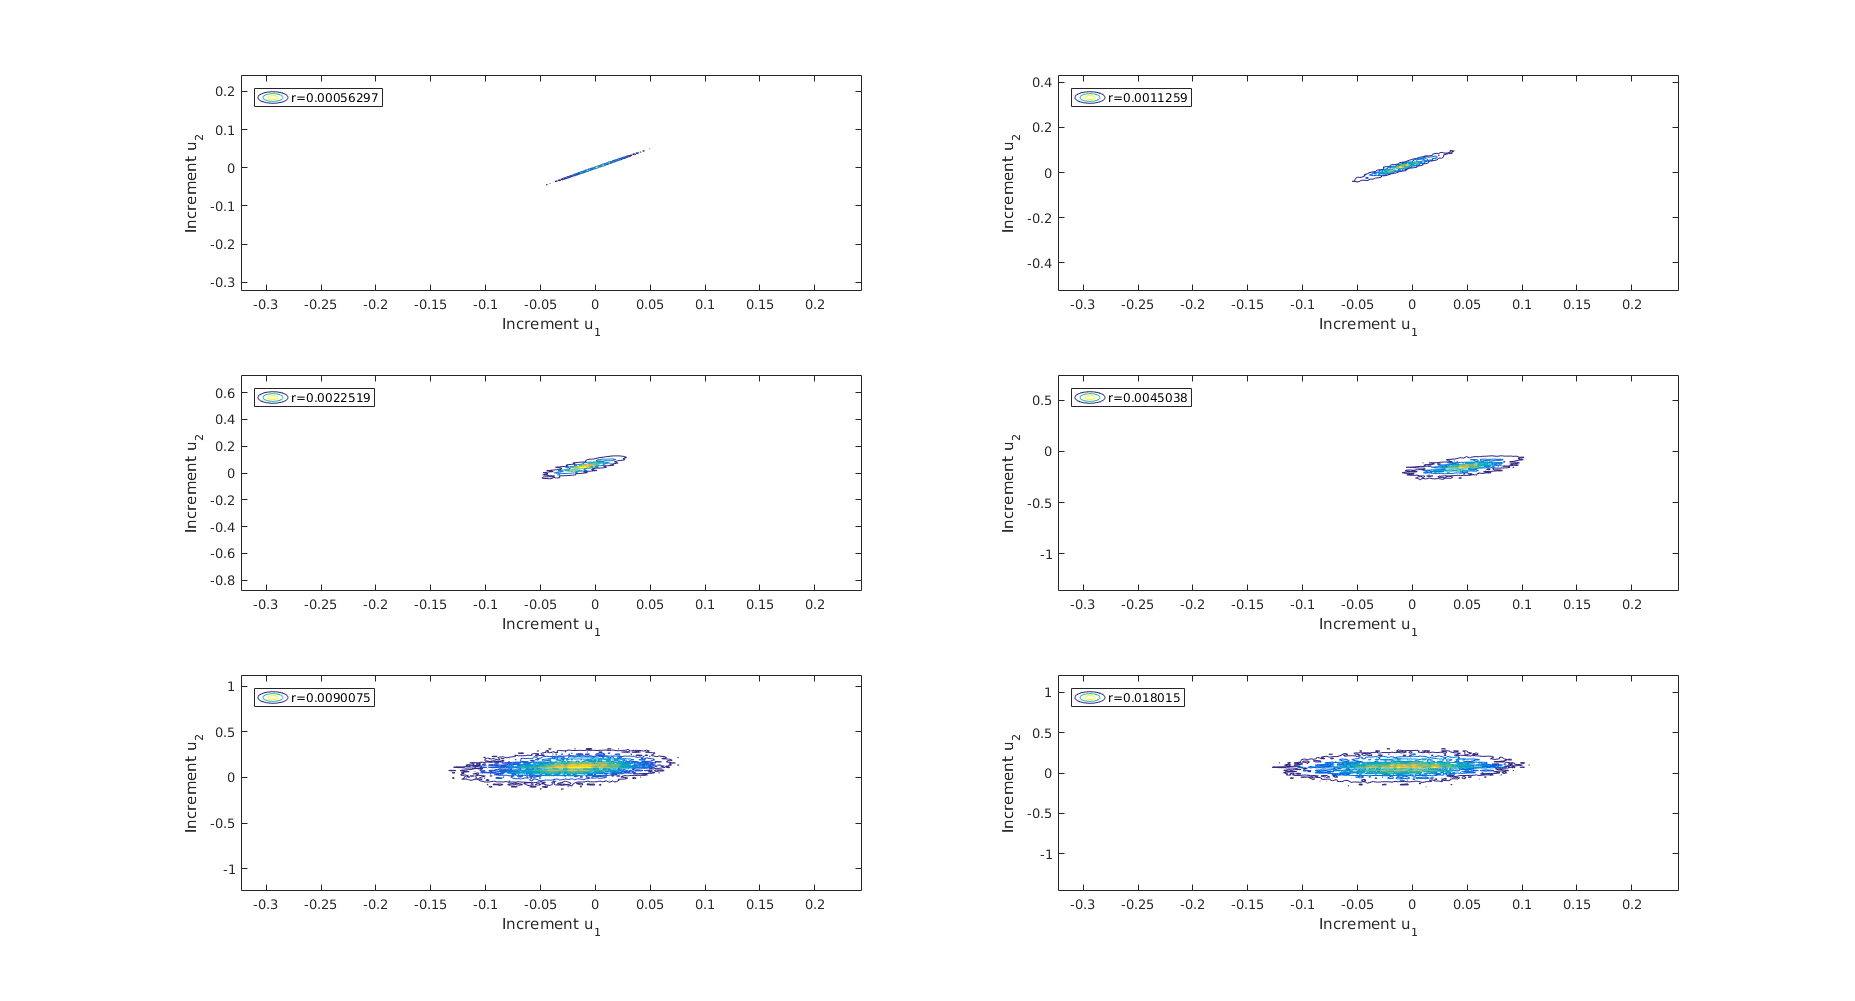
\includegraphics[width=1\linewidth]{figures/labdata_npoint.png}
\caption{Conditional PDF of JFM data with increasing time lag}
\label{fig:npoint_center}
\end{figure}
It can be seen that the correlation between the two wind speed increments decrease with increasing time lag. But there is a difference between the atmosphere dataset and the JFM dataset. Since the JFM data represents nearly ideal turbulence it can be seen that for homogeneous turbulence a stronger correlation between the wind increments can be identified.
\newpage
\section{References}
\bibliography{literature}
\bibliographystyle{apalike}
\end{document}